% ============================================================
% Arquitectura del sistema - App Turismo Comarapa
% Requiere en el preambulo del documento principal:
%   \usepackage{graphicx} % para \includegraphics
%   \usepackage{float}    % para el especificador de posicion [H]
%   \usepackage{array}    % para columnas p{} y el modificador >{\bfseries}
% Imagen asociada: DIAGRAMA_ARQUITECTURA.png / .svg / .pdf (misma carpeta)
% ============================================================

\subsection*{Arquitectura del sistema}

La arquitectura está compuesta por cuatro componentes principales: una
aplicación cliente (\textbf{frontend}) desarrollada en Flutter, un
\textbf{backend} basado en el modelo Backend-as-a-Service (BaaS) de
Supabase, una \textbf{base de datos} PostgreSQL gestionada por el mismo
Supabase, y un conjunto de \textbf{servicios externos} (Open-Meteo, OpenStreetMap,
OSRM y el sensor GPS nativo del dispositivo). Estos componentes se
comunican principalmente mediante \textbf{peticiones HTTPS} con
intercambio de datos en formato \textbf{JSON}: el frontend consume la
API REST autogenerada de Supabase (PostgREST) a través del SDK
\texttt{supabase\_flutter}, adjuntando el token de sesión (JWT) emitido
por Supabase Auth en cada operación que lo requiere; de forma paralela,
el frontend consume directamente, también por HTTPS/REST, las APIs de
clima (Open-Meteo) y de ruteo (OSRM), y obtiene las teselas del mapa
interactivo desde OpenStreetMap, mientras que la ubicación del usuario
se obtiene mediante acceso nativo al sensor GPS del dispositivo (no es
una llamada de red). El componente de \textbf{presentación} (frontend)
es responsable de renderizar la interfaz de usuario, capturar la
interacción del turista y del administrador, gestionar el estado local
de la aplicación (mediante \texttt{Provider}) y mantener una caché local
de contingencia (``Plan B Offline'') con \texttt{shared\_preferences}
para los casos sin conexión. El \textbf{backend} gestiona la
autenticación y las sesiones de usuario (Supabase Auth), aplica las
reglas de autorización por rol mediante políticas de \emph{Row Level
Security} (RLS) que distinguen entre los roles ``editor'' y
``administrador'', expone los datos turísticos a través de la API REST
generada automáticamente sobre la base de datos, y administra el
almacenamiento de imágenes (Supabase Storage) referenciadas por URL
pública. Finalmente, la capa de \textbf{persistencia} almacena los datos
estructurados del sistema: perfiles de usuario y su rol
(\texttt{usuarios}), el catálogo de categorías por módulo
(\texttt{categorias}), el contenido turístico (\texttt{lugares},
\texttt{hoteles}, \texttt{restaurantes}, \texttt{actividades},
\texttt{gastronomia}, \texttt{eventos}) y las reseñas y calificaciones
de los usuarios, estas últimas sujetas a un flujo de moderación
(\texttt{pendiente}, \texttt{aprobada}, \texttt{rechazada}).

\begin{figure}[H]
\centering
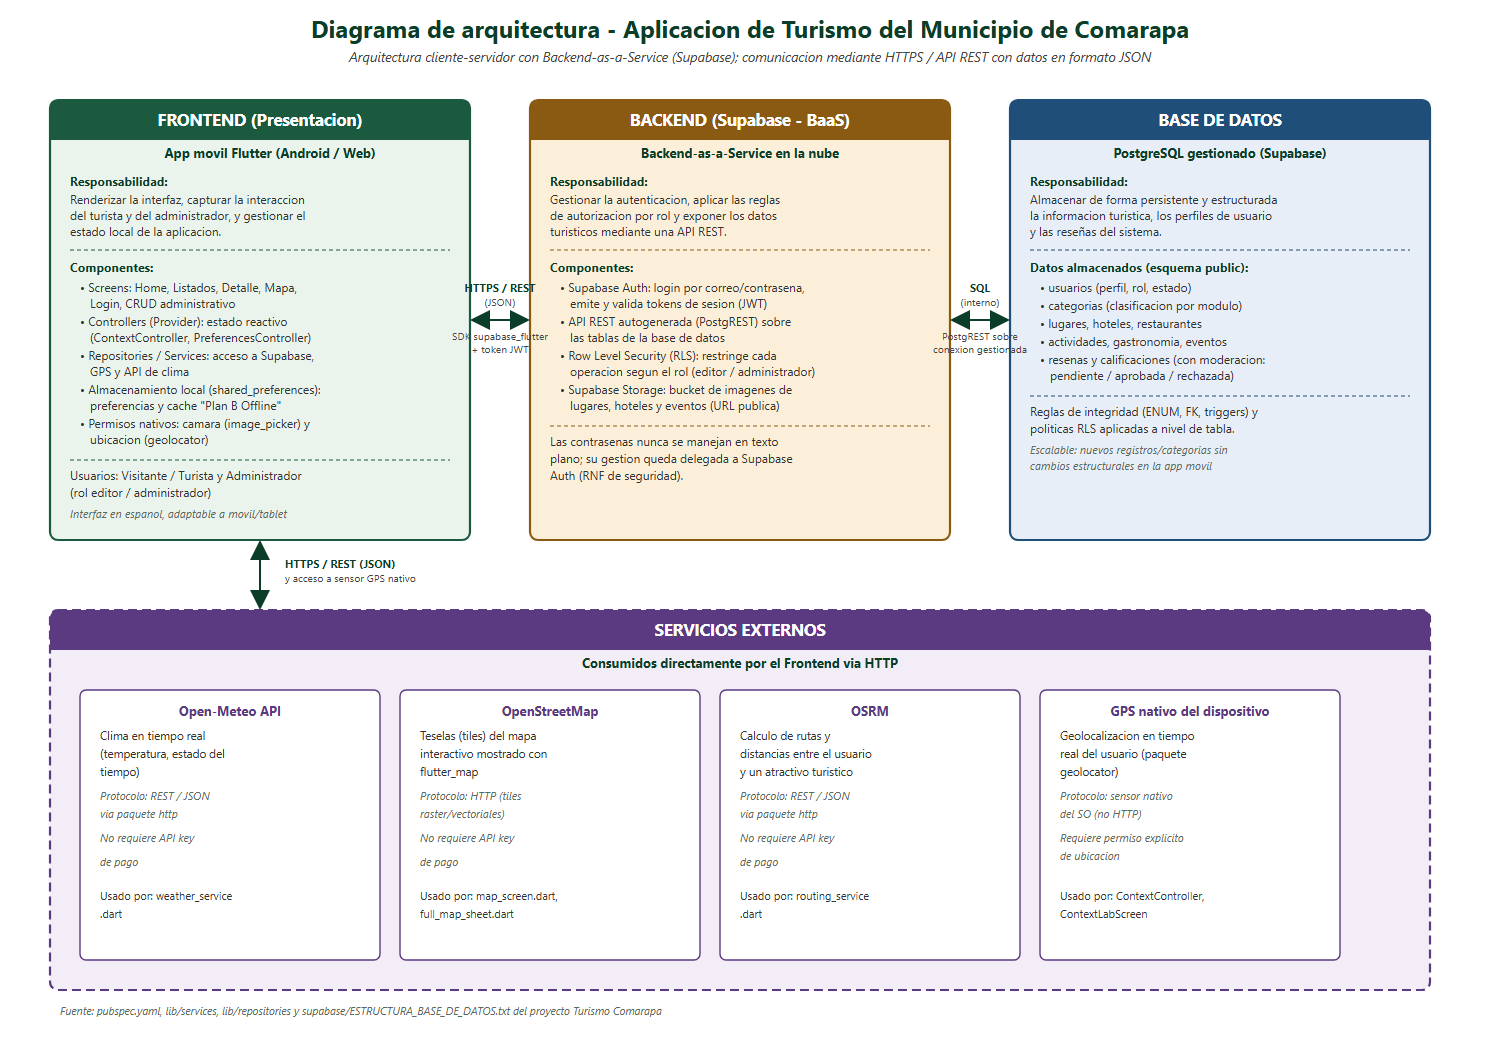
\includegraphics[width=\textwidth]{DIAGRAMA_ARQUITECTURA.png}
\caption{Diagrama de arquitectura de la aplicación de turismo del municipio de Comarapa}
\label{fig:arquitectura}
\end{figure}

\begin{table}[H]
\centering
\caption{Resumen de responsabilidades por capa}
\label{tab:arquitectura}
\renewcommand{\arraystretch}{1.3}
\begin{tabular}{|>{\bfseries}p{2.6cm}|p{4.0cm}|p{6.9cm}|}
\hline
Capa & Tecnología & Responsabilidad principal \\ \hline

Presentación (frontend) & Flutter (Android / Web) &
Interfaz de usuario, captura de interacción, estado local (Provider) y
caché offline (shared\_preferences). \\ \hline

Backend & Supabase (BaaS): Auth, PostgREST, Storage &
Autenticación, autorización por rol (RLS), exposición de la API REST y
almacenamiento de imágenes. \\ \hline

Base de datos & PostgreSQL (gestionado por Supabase) &
Persistencia de usuarios, categorías, contenido turístico y
reseñas/calificaciones con moderación. \\ \hline

Servicios externos & Open-Meteo, OpenStreetMap, OSRM, GPS nativo &
Clima en tiempo real, teselas de mapa, cálculo de rutas y
geolocalización del usuario. \\ \hline

\end{tabular}
\end{table}
